\documentclass[letterpaper,man,natbib,noextraspace,floatsintext,longtable]{apa6}  

\usepackage[english]{babel}
\usepackage[utf8x]{inputenc}
\usepackage{amsmath}
\usepackage{graphicx}
\usepackage{booktabs}             % fancy latex tables
\usepackage[export]{adjustbox}    % center wide tables on page
\usepackage{setspace}             % adjust caption linespacing 
\usepackage{multibib}             % references in supplement
\usepackage{hyperref}             % manage hyperlink colors

% override apa6 section headers
% https://tex.stackexchange.com/questions/125537/how-to-modify-subsubsection-header-apa6-cls
\makeatletter
\renewcommand{\subsubsection}{\@startsection{subsubsection}{3}
  {\z@}%
  {\b@level@two@skip}{\e@level@two@skip}%
  {\normalfont\normalsize\bfseries}}
\makeatother

% center contents of longtable
\usepackage{array}
\newcolumntype{P}[1]{>{\centering\arraybackslash}p{#1}}

% setup supplementary references
\newcites{SM}{Supplementary references}

% decrease size of references (lol)
\renewcommand*{\bibfont}{\small}

% change hyperlink colors
\hypersetup{
    colorlinks=true,
    linkcolor=blue,
    filecolor=magenta,      
    urlcolor=cyan,
    citecolor=blue
}

\title{The MACE is essentially unidimensional: Bifactor models of the `Maltreatment and Abuse Chronology of Exposure' scale}
\shorttitle{Bifactor models of MACE}
\author{Samuel Zorowitz$^1$, Lauri Tuominen$^{2}$}
\affiliation{$^1$Princeton Neuroscience Institute, Princeton University, USA\\$^2$The Royal’s Institute of Mental Health Research, University of Ottawa, Canada}

\abstract{

\textbf{Background}: Typically measures of childhood maltreatment collect information about several types of abuse and maltreatment. The subscales of the retrospective Maltreatment and Abuse Chronology of Exposure (MACE) scale measure 10 such types. Since different types of maltreatment often co-occur, it is not clear whether subscale measures can be used to reflect constructs unique from from overall maltreatment.

\hfill 

\textbf{Methods}: Here, we investigated the factor structure of the MACE scale in two independent samples (N=1051 \& N=582). We used both confirmatory and exploratory item response modeling.

\hfill

\textbf{Results}: We found the MACE total score to be a reliable and valid measure of general maltreatment. Confirmatory item response models provided strong evidence for unidimensionality of the MACE, with the exception of a potential peer victimization factor. That is, most items in the MACE load on general factor and apart from peer victimization very little variance was explained by other subscales. Exploratory factor modeling further supported these findings. 

\hfill

\textbf{Conclusions}: The MACE is essentially a unidimensional scale. Apart from a separate peer victimization factor, researchers should refrain from using subscales data separately since they mostly reflect overall maltreatment.  
\hfill \break
}

\keywords{child maltreatment, reliability, item response theory, bifactor model}

\authornote{This work was funded in part by an NSF Graduate Research Fellowship. The authors have no conflicts of interest to declare.}

\begin{document}

\maketitle

\section{Introduction}

Childhood maltreatment is an unfortunately common experience for children across the globe \citep{stoltenborgh2015prevalence}. It is a risk factor for multiple poor outcomes later in life including the development of mental illness \citep{kessler2010childhood}, challenges in cognitive functioning \citep{su2019does}, and poor physical health \citep{wegman2009meta}. Childhood maltreatment also predicts worse treatment outcomes for several psychiatric disorders \citep{nanni2012childhood, thomas2019childhood}. Thus, reliable and valid assessment of childhood maltreatment is an important research goal in order to refine our understanding of the link between maltreatment and health outcomes; augment treatment strategies for victims of childhood maltreatment; and ultimately design better interventions to prevent maltreatment in the first place. 

There already exist many measures of childhood abuse and maltreatment for researchers to choose from \citep{saini2019systematic}. One recently developed measure, the Maltreatment and Abuse Chronology of Exposure scale (MACE; \citealt{teicher2015maltreatment}), has a number of notable advantages. The MACE is a 52-item retrospective self-report scale composed of 10 subscales, each of which measures a unique type of childhood maltreatment. Six of these subscales overlap with other standard measures of abuse (e.g. physical abuse, neglect), whereas the remaining four are less commonly represented in other scales (e.g. peer victimization, witnessing domestic violence). The items in the MACE were carefully selected to measure maltreatment of varying severity in order to finely differentiate people with differing exposure levels. The MACE also asks for the onset and duration of maltreatment experiences, which is necessary for investigating how the timing of abuse shapes development. The MACE was originally developed to provide two measures: a total score (number of overall maltreatment experiences) and a multiplicity score (number of types of maltreatment experienced). These scores have excellent temporal stability, convergent validity with other childhood maltreatment scales, and good predictive validity for a multitude of psychiatric symptoms \citep{teicher2015maltreatment}. For these reasons, the MACE has been included as among the best measures of childhood maltreatment currently available \citep{saini2019systematic, georgieva2022systematic}.

In recent years, there have been calls for childhood maltreatment research to move away from the cumulative risk framework \citep{evans2013cumulative} --- which focuses only on the number of adverse experiences --- towards a dimensional approach, which emphasizes how distinct types of maltreatment uniquely shape developmental trajectories \citep{mclaughlin2016beyond, belsky2012beyond}. In response, some researchers have begun to use the MACE to make new indices of maltreatment in lieu of, or in addition to, the total and multiplicity scores. For example, some have used all 10 MACE subscale scores to study the unique contributions of each type of maltreatment to the development of psychopathology \citep{schalinski2015type, gerke2018childhood, schalinski2019early}. Inspired by a prominent dimensional model of maltreatment \citep{mclaughlin2014childhood}, others have made new subscale scores indexing threat and deprivation experiences using the items in the MACE that respectively measure abuse and neglect \citep{schalinski2018defining, schalinski2019environmental, teicher2018differential}. Yet the psychometric properties of these new subscale scores have not been thoroughly investigated.   

A critical challenge in studying the consequences of childhood maltreatment is the high co-occurrence of these adverse experiences. That is, children who have experienced any single form of maltreatment are likely to have experienced multiple other types \citep{dong2004interrelatedness, herrenkohl2009assessing, kessler2010childhood}. As a consequence, isolating the unique contribution of one type of maltreatment to some outcome is difficult insofar as any one type of adversity is likely confounded with overall maltreatment. Concretely, this means that researchers intending to study the effects of particular types of maltreatment using subscale scores need to verify that those measures actually reflect a construct unique from from overall maltreatment, lest they risk drawing spurious conclusions.

Bifactor models, a type of hierarchical factor model, are well-suited for addressing this issue \citep{bornovalova2020appropriate}. They assume that the covariation in responses to a set of items can be accounted for by a \emph{general} factor, reflecting shared variance across all items, and one or more \emph{specific} factors, reflecting additional shared variance among subsets of items \citep{Reise2012-ql}. Crucially, bifactor models can be used to calculate model-based reliability statistics, including the omega hierarchical ($\omega_h$) and omega subscale ($\omega_s$) indices \citep{reise2013scoring}, which respectively measure the proportion of variance in total and subscale scores attributable to the general factor and specific factors. Applied to the MACE, these indices can help determine if subscale scores measuring particular types of maltreatment are interpretable as such, or if they instead primarily reflect overall maltreatment. 

In this study, we investigated the factor structure of the MACE in two independent samples of participants. First, we tested the fits of a series of confirmatory item response models to the maltreatment data from each sample. These included several bifactor models, which allowed us to quantify the proportion of variance in the data attributable to general maltreatment versus specific types of abuse. We found that the MACE is essentially unidimensional; that is, the majority of reliable variance in participants' responses was attributable to a general maltreatment factor. We then calculated the reliability of the MACE total score and a host of subscale scores. We found the total score was a reliable and valid measure of general maltreatment, whereas most subscale scores contained little-to-no variance unique from general maltreatment. The only possible exception to this trend was for a novel peer victimization subscale. Finally, we performed exploratory factor analysis to examine the factor structure of the MACE without \textit{a priori} restrictions. These analyses supported the results of the confirmatory factor analyses. 

\section{Methods}

All data, code, and analysis materials are publicly available at \url{https://github.com/szorowi1/mace-irt}.

{\begin{spacing}{0.2} \hfill \\ \end{spacing}} \subsection{Participants}

The participants in the current study (N=1633 total) belonged to one of two samples. The first sample of participants (N=1051) are from the original development of the MACE \citep{teicher2015maltreatment}. The full recruitment details for this sample have been reported elsewhere \citep{teicher2015maltreatment}. Briefly, these participants were recruited from the greater Boston area between 2010 and 2013. Inclusion criteria included being medically healthy, unmedicated, and between 18–25 years of age. This sample will hereafter be referred to as the \textit{original} sample. 

The second sample of participants (N=687) were recruited from the Prolific Academic platform (\url{https://www.prolific.co}) to participate in an online experiment in August -- October, 2021. Of these, N=582 were retained for analysis (see Exclusion Criteria below). Participants were eligible for participation if they were 18 years or older and currently resided in the United States or Canada. Participants received monetary compensation for their time (rate: \$12 USD/hr). This study was approved by the Institutional Review Board of the University of Ottawa (\#2021003), and all participants provided informed consent. This sample will hereafter be referred to as the \textit{replication} sample. 

\begin{table}[t!]
    \centering
    \begin{tabular*}{\textwidth}{lccc}
    \toprule
    Variable & Original (N=1051) & Replication (N=582) & p-value \\
    \midrule
    \textbf{Gender}, N (\%)                & & & p < 0.001 \\
    \hspace{1em} Women                     & 670 (63.7\%) & 310 (53.3\%) & \\
    \hspace{1em} Men                       & 381 (36.3\%) & 258 (44.3\%) & \\
    \hspace{1em} Trans or NB               &   0  (0.0\%) &   9  (1.5\%) & \\
    \hspace{1em} Rather not say            &   0  (0.0\%) &   5  (0.9\%) & \\
    \midrule
    \textbf{Age}, yrs                      & & & p < 0.001 \\
    \hspace{1em} Mean (range)              & 23.1 (18 -- 27) & 30.2 (18 -- 80) & \\
    \midrule
    \textbf{Ethnicity}, N (\%)             & & & p = 0.214 \\
    \hspace{1em} Not Hispanic or Latino    & 963 (91.6\%) & 518 (89.0\%) & \\
    \hspace{1em} Hispanic or Latino        &  84  (8.0\%) &  57  (9.8\%) & \\
    \hspace{1em} Rather not say            &   4  (0.4\%) &   7  (1.2\%) & \\
    \midrule
    \textbf{Race}, N (\%)                  & & & p = 0.677 \\
    \hspace{1em} White                     & 806 (76.7\%) & 441 (75.8\%) & \\ 
    \hspace{1em} Asian                     & 103  (9.8\%) &  65 (11.2\%) & \\
    \hspace{1em} Black or African American &  81  (7.7\%) &  31  (5.3\%) & \\
    \hspace{1em} Other                     &  61  (5.8\%) &  28  (4.8\%) & \\
    \hspace{1em} Rather not say            &   0  (0.0\%) &  17  (2.9\%) & \\
    \bottomrule
    \end{tabular*}
    \caption{\normalfont Demographics of the two samples included in this study. The original sample was recruited and reported by \cite{teicher2015maltreatment}. The replication sample was recruited by the current authors for the purposes of this study.}
    \label{tab:demographics}
\end{table}

The demographics of the two samples are summarized in Table \ref{tab:demographics}. The majority of participants in both samples identified as women, though the original sample was composed of proportionally more woman than the replication sample ($z$ = 4.142, $p$ < 0.001). Participants in the original sample were also younger on average ($t$ = -19.313, $p$ < 0.001). The majority of participants in both samples identified as White and not as Hispanic or Latino. The proportion of participants identifying as White was not significantly different across samples ($z = 0.417$, $p = 0.677$), nor was the proportion of participants identifying as Hispanic or Latino ($z$ = -1.241, $p$ = 0.214).

{\begin{spacing}{0.2} \hfill \\ \end{spacing}} \subsection{Measures}

All participants completed the 52-item version of the MACE \citep{teicher2015maltreatment}. The MACE is a retrospective self-report scale that measures 10 unique types of childhood maltreatment (i.e. parental verbal abuse, physical abuse, nonverbal emotional abuse, sexual abuse, emotional neglect, physical neglect, witnessing violence to siblings, witnessing interparental violence, peer verbal abuse, peer physical abuse). For each item, participants endorse whether they ever experienced a particular event during childhood (e.g. ``Parents or guardians intentionally pushed, grabbed, shoved, slapped, pinched, punched or kicked you'') and, if so, at what ages (up to age 18). Here we only analyze the dichotomous endorsement responses (Yes = 1, No = 0) and not the chronology data. Six of the 52-items --- evenly divided between the emotional and physical neglect subscales --- are positively valenced and reverse-scored (e.g. ``One or more individuals in your family helped you feel important or special''). For these items we follow the scoring convention set by \cite{teicher2015maltreatment}: a score of 1 is assigned to a response only in the absence of a positive event for all 18 years of childhood. This is in contrast to the remaining items in the scale, where a score of 1 is assigned to a response if maltreatment or abuse occurred in at least one year of childhood.

In both the original and replication samples, participants completed a number of additional self-report symptom measures. We do not include these in our analyses and therefore do not discuss these measures further in the main text. For completeness, we report these secondary self-report measures in the supplementary materials. 

{\begin{spacing}{0.2} \hfill \\ \end{spacing}}  \subsection{Exclusion criteria}

To ensure data quality in the replication sample, we relied on attention checks embedded in the self-report measures to identify and remove participants engaging in careless or insufficient effort responding (\citealt{zorowitz2021inattentive}; see the supplementary materials for the attention checks). The data from N=64 (9.9\%) participants in the replication sample were excluded for failing one or more of these attention checks, leaving the data from N=582 participants for analysis.

{\begin{spacing}{0.2} \hfill \\ \end{spacing}} \subsection{Differential item functioning}

Prior to analysis, we investigated whether it was appropriate to combine response data from the original and replication samples. We first compared maltreatment endorsement rates for each item between samples. The Spearman-rank correlation of endorsement rates across samples was large ($\rho$ = 0.951, p < 0.001), indicating excellent correspondence in the relative prevalence of maltreatment types across samples. When we compared the distribution of person-level total scores across samples, however, we found that scores were greater on average in the replication sample than in the original sample ($p_1$ = 0.185, $p_2$ = 0.219, $t$ = -4.611, p < 0.001). 

An overall shift in overall endorsement rates by sample is not necessarily evidence for a violation of measurement invariance. One possibility is that the replication sample had simply experienced more adversity than the original sample. A second is that the differences in the demographic composition of the two samples (e.g. gender, age) explain the differences in endorsement rates. To investigate these possibilities, we tested for uniform differential item functioning (DIF) using logistic regression, in which a participant's endorsement response on an item is regressed against their rest score (i.e. their total score for all other items), sample membership, gender, and age.

Using the cutoffs recommended by \cite{hidalgo2014binary}, we identified 11 of 52 items on the MACE with large DIF by study (Figure \ref{fig:dif_study}). These included all six reverse-scored items. We also found an additional 11 items with large DIF by gender (Figure \ref{fig:dif_gender}). Five of these items measured sexual abuse (endorsed more frequently by women), and another five measured peer physical abuse (endorsed more frequently by men). We identified no items that exhibited large DIF by age. Given the number of items with DIF by sample membership, we decided to analyze each sample separately.

{\begin{spacing}{0.2} \hfill \\ \end{spacing}} \subsection{Response dependence}

The MACE contains a total of 12 item pairs and triplets characterized by response dependence (Table \ref{tab:dependence}). The items in some of these sets are structurally dependent, where a response to one item requires or strongly implies a certain response on the second. For example, a person endorsing item 8 (``Parents or guardians hit you so hard that you received medical attention'') is all but certain to endorse item 7 (``Parents or guardians hit you so hard that it left marks for more than a few minutes''). Other items are dependent by virtue of redundancy. One such example is items 36 (``Peers forced you to engage in sexual activity against your will'') and 37 (``Peers forced you to do things sexually that you did not want to do``); here the same question is asked twice using slightly different language.

We were concerned about response dependence for two reasons. First, it can inflate the estimates of item discrimination parameters, making items appear more informative than they actually are \citep{marais2008formalizing}. Second, response dependence can inflate the estimates of item loadings on specific factors in bifactor models, giving false support for models with a greater number of factors than needed \citep{reise2013applying}. Following \cite{marais2008formalizing}, we therefore converted each set of dependent items into a single polytomous item thereby reducing the MACE from 52 to 39 items in total.

{\begin{spacing}{0.2} \hfill \\ \end{spacing}} \subsection{Confirmatory item factor models}

To investigate the factor structure of the MACE, we fit a series of confirmatory item factor models separately to the response data from each sample. The basis of each model is the graded response model for ordered polytomous data \citep{samejima1997graded}. The factor structure for each of the four models is depicted in Figure \ref{fig:models}. The first model is a one-factor (undimensional) model where all items load onto a general maltreatment factor (Figure \ref{fig:models}a). The second is a bifactor model where all items load onto a general maltreatment factor and also one of 10 specific factors based on their subscale membership (Figure \ref{fig:models}b). This model will be used to evaluate if the MACE can produce reliable subscale scores for each of the 10 types of maltreatment assessed by the MACE. 

The third model was motivated by a theoretical account of childhood maltreatment that distinguishes between threat and deprivation experiences as distinct types of adversity \citep{mclaughlin2014childhood}. To explore this model of the MACE, we initially fit a bifactor model where all items loaded onto a general maltreatment factor, and also a threat or neglect specific factor. However, we observed vanishing item loadings on the threat specific factor. As such, we instead fit a bifactor S-1 model \citep{eid2017anomalous} where all items load onto a general maltreatment factor, and only items measuring neglect load onto a specific factor (Figure \ref{fig:models}c). This model will be used to evaluate if the MACE can produce reliable neglect subscale scores distinguishable from general maltreatment. 

\begin{figure}[t!]
    \centering
    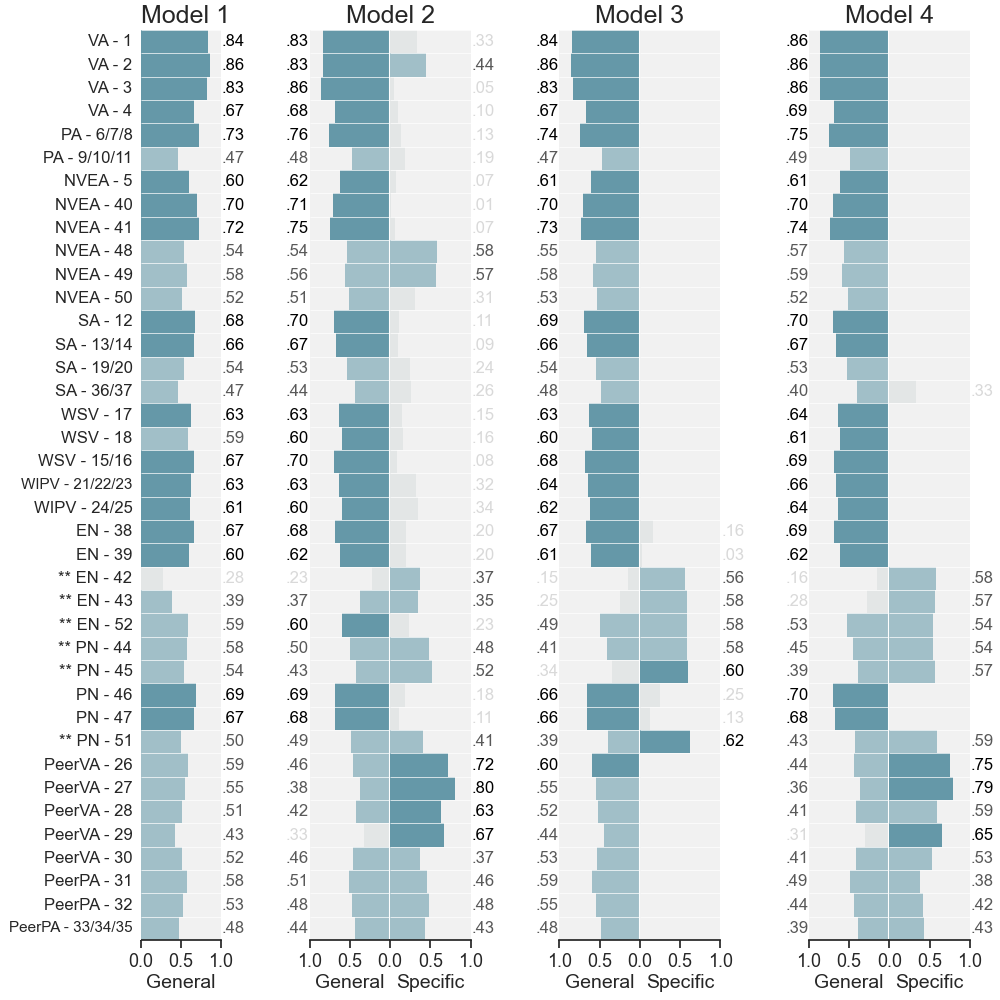
\includegraphics[width=1.1\textwidth,center]{figures/fig01.png}
    \captionsetup{width=1.1\textwidth}
    \caption{\normalfont The structure of the four competing confirmatory factor models of the MACE. (A) One-factor (unidimensional) model. (B) Bifactor model with 10 specific factors (one per MACE subscale). (C) Bifactor S-1 model with 1 specific factor (neglect). (D) Bifactor S-1 model with 2 specific factors (peer victimization, reverse-scoring). Notes: G = general maltreatment; VA = verbal abuse; PA = physical abuse; NVEA = nonverbal emotional abuse; SA = sexual abuse; WSV = witnessing sibling vioence; WIPV = witnessing inter-parental violence; EN = emotional neglect; PN = physical neglect; PeerVA = peer verbal abuse; PeerPA = peer physical abuse.}
    \label{fig:models}
\end{figure}

The fourth and final model proposes a more parsimonious structure of the MACE based on the content of its items. Items on the MACE can be organized according to the source of maltreatment: parents (or other adults in the home) and peers. Thus, we hypothesized there would be two factors underlying responses on the MACE: a primary maladaptive parenting factor and a secondary peer victimization factor. Based on preliminary model fitting, we also suspected the presence of a tertiary methods factor affecting the six reverse-scored items. We initially fit a bifactor model in which all items loaded onto a general maltreatment factor and one of three specific factors (maladaptive parenting, peer victimization, reverse-scoring); however, we observed vanishing loadings on the first specific factor. As such, we instead fit a bifactor S-1 model where all items load onto a general maltreatment factor, and the peer victimization \& reverse-scoring items additionally load onto their own specific factors (Figure \ref{fig:models}d). This model will be used to evaluate if the MACE can produce peer victimization reliable subscale scores distinguishable from general maltreatment. 

All confirmatory item factor models were estimated within a Bayesian framework using Hamiltonian Monte Carlo as implemented in Stan (v2.26; \citealt{carpenter2017stan}). For each model, four separate chains with randomized start values each took 3,000 samples from the posterior. The first 2,000 samples from each chain were discarded, so that 4,000 post-warmup samples from the posterior were retained. The $\hat{R}$ values for all parameters were less than 1.01, indicating acceptable convergence between chains, and there were no divergent transitions in any chain. 

{\begin{spacing}{0.2} \hfill \\ \end{spacing}} \subsection{Goodness of fit \& model comparison}

We relied on multiple indices to judge the fit of the models to the data. First we calculated three traditional goodness-of-fit statistics using the ordinal $M_2$ statistic \citep{cai2013limited}. $M_2$ is asymptotically $\chi^2$-distributed with $\kappa − \nu$ degrees of freedom ($df$), where $\kappa$ is the reduced number of first- and second-order marginal residuals (i.e. $\kappa = n(n + 1)/2$ for $n$ items) and $\nu$ denotes the number of free parameters. To improve the stability of the $M_2$ statistic, the responses to polytomous items were binarized (i.e. none vs. any maltreatment). Using the $M_2$ statistic, we calculated the root mean square error of approximation (RMSEA), comparative fit index (CFI), and Tucker-Lewis index (TLI) for each model fit. Following convention \citep{hu1999cutoff}, the benchmarks for adequate model fit are RMSEA < 0.08, CFI > 0.90, and TLI > 0.90; in turn, the benchmarks for good model fit are RMSEA < 0.05, CFI > 0.95, and TLI > 0.95. 

Given the limitations of SEM-based fit indices for item response models (e.g. \citealt{reise2014evaluating}), we calculated two additional fit indices. First, we used posterior predictive model checking to calculate a $\chi^2_{NC}$ discrepancy measure based on the total score distribution \citep{sinharay2006posterior}. This measure compares the observed and model-predicted proportion of participants at each total score level. Second, to test for local dependence in each pair of items, we calculated Yen's $Q_3$ statistic \citep{yen1984effects} and also the critical $Q_3$-value (i.e. the value above which local dependence is indicated; \citealt{christensen2017critical}). For each model and sample, we simulated 1000 locally independent datasets using the posterior distribution of the model parameters. We then recorded the maximum $Q_3$ value per simulation. The critical $Q_3$-value was defined as the 99th percentile of these max $Q_3$ values. 

The goodness-of-fit of the models was compared using Bayesian leave-one out cross- validation (LOO-CV; \citealt{vehtari2017practical}). The LOO-CV measure quantifies the discrepancy between the model and data while taking into account model complexity. LOO-CV values are presented in deviance scale, i.e. smaller values indicate better fit.

{\begin{spacing}{0.2} \hfill \\ \end{spacing}} \subsection{Model-based reliability indices}

To evaluate the reliability of the MACE total and subscale scores, we calculated several model-based reliability indices using the factor loadings from the bifactor models. First, we calculated coefficient omega ($\omega$; \citealt{mcdonald2013test}), which quantifies the proportion of reliable score variance attributable to all factors (i.e. both general and specific factors). Next we calculated coefficient omega hierarchical ($\omega_h$) and coefficient omega subscale ($\omega_s$;  \citealt{reise2013scoring}). Whereas $\omega_h$ measures the fraction of total score variance attributable to the general factor, $\omega_s$ measures the fraction of subscale score variance attributable to a specific factor after controlling for the general factor. The values of $\omega_h$/$\omega_s$ facilitate interpretation of total and subscale scores. Values of $\omega_h$ approaching 1 indicate the general factor is the primary source of reliable variance in a total score. When $\omega_h$ > 0.80, the total score may be considered an essentially unidimensional reflection of the general factor \citep{rodriguez2016applying}. Values of $\omega_s$ approaching 1 indicate the specific factor, not the general factor, is the primary source of reliable variance in a subscale score. \cite{canivez2016bifactor} suggested that an acceptable $\omega_s$ value is 0.50 and that >0.70 is desirable. In contrast, values of $\omega_s$ < 0.50 preclude the interpretation of subscale scores as primarily reflecting a specific factor \citep{gignac2013bifactor}. 

To assess the unidimensionality of the MACE, we calculated the explained common variance (ECV; \citealt{sijtsma2009use}) and the proportion of uncontaminated correlations (PUC; \citealt{reise2013multidimensionality}). The ECV is the ratio of the variance explained by the general factor divided by the total common variance of a scale. It thus measures the contribution of the general factor relative to the specific factors. As ECV values approach 1, the general factor loadings of a bifactor model are expected to resemble the item loadings that would be obtained by a one-dimensional model. ECV values greater than 0.70 often indicate a scale is essentially unidimensional \citep{rodriguez2016applying}. In turn, PUC quantifies how many inter-item correlations are accounted for only by the general factor. PUC is an important moderator of the ECV; as PUC increases, ECV is less important for evaluating the risk of bias when fitting a unidimensional model to data with a latent bifactor structure. When PUC > 0.80, there is a low risk of bias when a multi- dimensional scale is treated as unidimensional \citep{reise2013multidimensionality}. We also calculated the relative parameter bias (RPB), which is the difference between an item's loading in a unidimensional model and its corresponding general factor loading in a bifactor model, divided by the general factor loading from the bifactor model. RPB less than 10–15\% is acceptable \citep{muthen1987structural}.

Finally, we calculated the H index to assess the construct replicability of each factor \citep{hancock2001rethinking}. The H index is an estimate of how well a set of items represents a latent factor. H values closer to 1 indicate a well-defined latent factor with item loadings more likely to be stable across studies. In contrast, small H values suggest a poorly defined latent factor where item loadings are liable to change across studies. Because we are presently focused on evaluating the reliability of MACE total and subscale scores, we report the H values below but do not interpret them further.

{\begin{spacing}{0.2} \hfill \\ \end{spacing}} \subsection{Exploratory factor analysis}

In addition to confirmatory factor analysis, we also performed exploratory factor analysis (EFA) on the response data from each sample separately. The goal of the EFA was to examine what factor structure would emerge with no \emph{a priori} restrictions placed on the data. We decided to extract two- and three- factor solutions based on the total number of factors in the bifactor S-1 models. We were particularly interested to see if a two-factor solution would reproduce the factors from model 3 (threat, deprivation); and if a three- factor solution would reproduce the three factors from model 4 (parental maltreatment, peer victimization, reverse-scoring). 

EFA was performed using the \textit{lavaan} (v0.6.11; \citealt{lavaan}) package available in R. Factors were extracted using the oblique geomin \citep{yates1987multivariate} and cf-quartimax rotation criteria \citep{crawford1970general}, which were selected in order to extract simple factor structures with few cross-loadings. We used two rotation criteria in order to examine the generalizability of the factor solutions across rotations. We again relied on traditional fit indices (i.e. RMSEA, CFI, TLI) to evaluate the goodness-of-fit of the exploratory factor models to the response data of both samples.

\section{Results}

\subsection{Goodness-of-fit \& model comparison}

The goodness-of-fit indices for each model and sample are summarized in Table \ref{table:cfa_diagnostics}. According to the traditional indices, each model provided at least an acceptable fit to the data. All RMSEA value were <0.05 and most CFI and TLI values were >0.95. The only exception were for the fits of models 1 and 3 to the original sample data where CFI \& TLI > 0.90. In general, model fits were better for the replication sample data than for the original sample. Furthermore, none of the posterior predictive p-values corresponding to the $\chi^2_{NC}$ discrepancy measure exceeded the critical values indicating that all models were able to reproduce the observed distribution of total scores for each sample.

\begin{table}[t!]
\small
\centering
\begin{adjustbox}{center}
\begin{tabular}{ccccccccccr}
\toprule
Sample & Model & $\chi^2 (df)$ &  RMSEA & CFI & TLI & $\chi^2_{NC}$ (PPP) & $Q3_{\max}$ &  $Q3_{\text{crit}}$ & LOO-CV & \multicolumn{1}{c}{$\Delta$LOO (se)} \\
\midrule
Original & 1 &  1858 (702) &  0.040 &  0.927 &  0.923 &  0.051 (0.230) &  0.589 &  0.239 &  30967.2 &  1748.0 (76.7) \\
& 2 &  1373 (663) &  0.032 &  0.955 &  0.950 &  0.046 (0.356) &  0.573 &  0.300 &  29211.3 & \multicolumn{1}{c}{-} \\
& 3 &  1571 (692) &  0.035 &  0.944 &  0.940 &  0.051 (0.214) &  0.591 &  0.255 &  30531.1 &  1312.0 (68.0) \\
& 4 &  1253 (687) &  0.028 &  0.964 &  0.961 &  0.046 (0.346) &  0.591 &  0.279 &  29219.2 & 7.9 (56.3) \\
\midrule
Replication & 1 &  1086 (702) &  0.031 &  0.954 &  0.952 &  0.065 (0.629) &  0.513 &  0.250 &  19771.6 &  1089.3 (58.4) \\
& 2 &   956 (663) &  0.028 &  0.965 &  0.961 &  0.058 (0.766) &  0.456 &  0.310 &  18706.2 &    24.0 (52.0) \\
& 3 &   881 (692) &  0.022 &  0.977 &  0.976 &  0.062 (0.684) &  0.468 &  0.316 &  19177.7 &   495.5 (45.0) \\
& 4 &   842 (687) &  0.020 &  0.982 &  0.980 &  0.058 (0.756) &  0.437 &  0.318 &  18682.2 & \multicolumn{1}{c}{-} \\
\bottomrule
\end{tabular}
\end{adjustbox}
\captionsetup{width=1\textwidth}
\caption{\normalfont Fit statistics for the confirmatory factor models by sample. LOO-CV values are presented in deviance scale (i.e. smaller values indicate better fit). Notes: RMSEA = root mean square error of approximation; CFI = comparative fit index; TLI = Tucker-Lewis index; PPP = posterior predictive p-value; $Q3_{\max}$ = maximum $Q_3$ value in the sample for the model; $Q3_{\text{crit}}$ = critical $Q_3$ value for the model; LOO-CV = leave-one-out cross-validation.}
\label{table:cfa_diagnostics}
\end{table}

Next we inspected the $Q_3$ indices for evidence of local dependence. For all models and samples, the maximum observed $Q_3$ index was greater than the critical $Q_3$ value. To gauge the extent of local dependence, we visualized the $Q_3$ values for item pairs exceeding the critical value for each model and sample (Figure \ref{fig:local_dependence}). The unidimensional model fits exhibited many locally dependent item pairs --- especially among the peer victimization and reverse-scored items --- suggesting possible underfactorization. By comparison, the three other models exhibited many fewer locally dependent item pairs. Of these pairs, the reasons for dependence were apparent. For example, the dependence between items 17 (``Parents made inappropriate sexual comments or suggestions to your sibling'') and 18 (``Parents touched or fondled your sibling in a sexual way'') observed in all models is almost certainly the result of measuring highly similar content. Regardless, the estimated item discrimination parameters for each model fit seldom exceeded the normal range ($\alpha \leq 4$). That is, the level of local dependence present in the models did not cause substantial bias in parameter estimation \citep{edwards2018diagnostic}. Thus, we conclude that all model fits provide at least an acceptable fit to the response data.

The results of the model comparison are also summarized in Table \ref{table:cfa_diagnostics}. Across samples, models 2 and 4 provided better fits to the data than models 1 and 3. Model 2 provided a numerically better fit to the data than model 4 in the original sample ($\Delta \text{LOO}$ = 7.9, se = 56.3), but the opposite was observed in the replication sample ($\Delta \text{LOO}$ = -24.0, se = 52.0). These differences in LOO-CV values, however, are both within four standard errors of the mean indicating only weak predictive improvements \citep{vehtari2022cv}. Thus the results suggest that models 2 and 4 provide approximately equal fits to the data, which is notable given that model 4 assumes a more parsimonious factor structure of the MACE.

{\begin{spacing}{0.2} \hfill \\ \end{spacing}} \subsection{Confirmatory item response models}

In the following sections, we interpret the fit of each confirmatory item response model. To facilitate interpretation, we have reproduced the standardized factor loadings of each model for the original sample in Figure \ref{fig:loadings_original} and for the replication sample in Figure \ref{fig:loadings_online}. The model-based reliability indices for the bifactor models are summarized in Table \ref{table:reliability}. 

{\begin{spacing}{0.2} \hfill \\ \end{spacing}} \subsubsection{Model 1: One-factor (unidimensional) model}

\begin{figure}[tp]
    \centering
    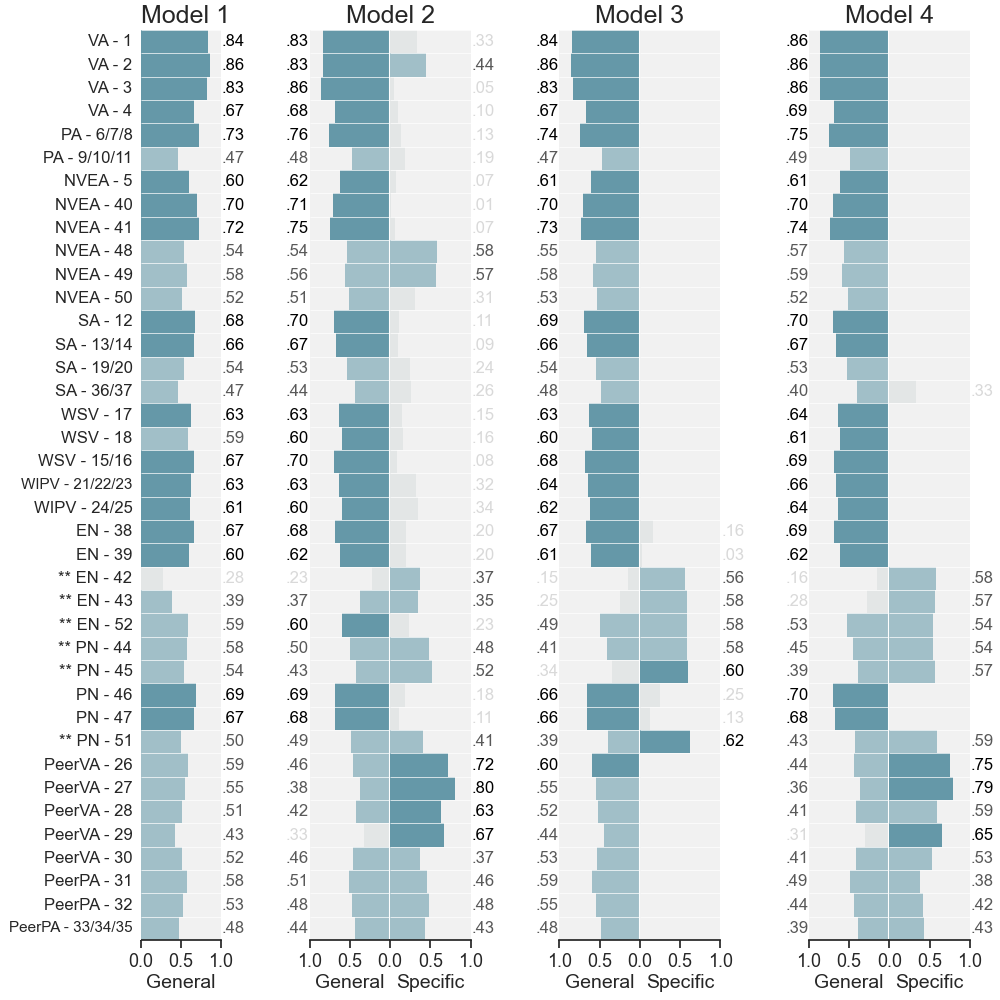
\includegraphics[width=1.1\textwidth,center]{figures/fig02.png}
    \captionsetup{width=1.1\textwidth}
    \caption{Standardized factor loadings from the four models fit to the original sample. Notes: Model 1 = one-factor (unidimensional) model; Model 2 = bifactor model with 10 specific factors; Model 3 = bifactor S-1 model with one specific factor (neglect); Model 4 = bifactor S-1 with two specific factors (peer victimization, reverse-scoring); VA = verbal abuse; PA = physical abuse; NVEA = nonverbal emotional abuse; SA = sexual abuse; WSV = witnessing sibling vioence; WIPV = witnessing inter-parental violence; EN = emotional neglect; PN = physical neglect; PeerVA = peer verbal abuse; PeerPA = peer physical abuse. Factor loadings $<$ 0.3 are displayed in gray; factor loadings $\geq$ 0.6 are bolded.  ** Reverse-scored items.}
    \label{fig:loadings_original}
\end{figure}

\begin{figure}[tp]
    \centering
    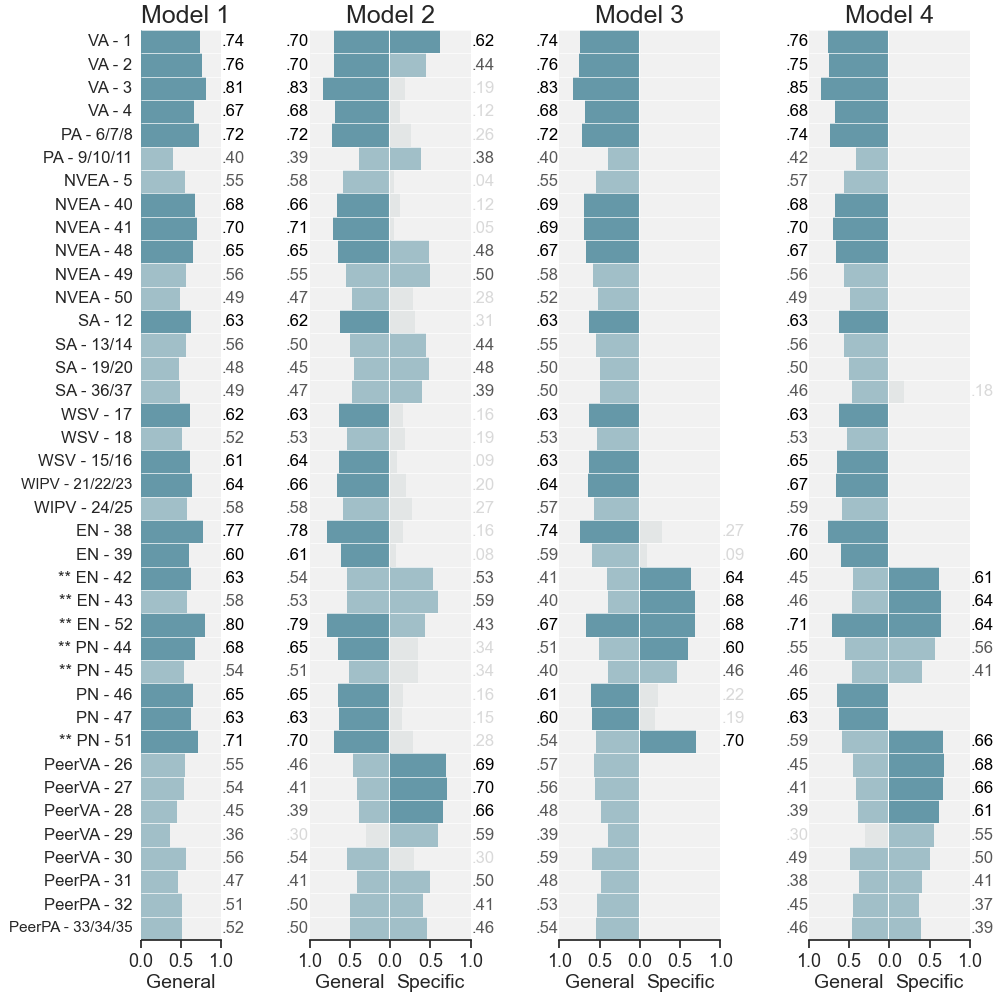
\includegraphics[width=1.1\textwidth,center]{figures/fig03.png}
    \captionsetup{width=1.1\textwidth}
    \caption{Standardized factor loadings from the four models fit to the replication sample. Notes: Model 1 = one-factor (unidimensional) model; Model 2 = bifactor model with 10 specific factors; Model 3 = bifactor S-1 model with one specific factor (neglect); Model 4 = bifactor S-1 with two specific factors (peer victimization, reverse-scoring); VA = verbal abuse; PA = physical abuse; NVEA = nonverbal emotional abuse; SA = sexual abuse; WSV = witnessing sibling vioence; WIPV = witnessing inter-parental violence; EN = emotional neglect; PN = physical neglect; PeerVA = peer verbal abuse; PeerPA = peer physical abuse. Factor loadings $<$ 0.3 are displayed in gray; factor loadings $\geq$ 0.6 are bolded.  ** Reverse-scored items.}
    \label{fig:loadings_online}
\end{figure}

The item discrimination parameters of the unidimensional model were, on average, large for both the original sample (mean $\alpha$ = 1.357, 95\% HDI = 1.295 -- 1.414) and replication sample (mean $\alpha$ = 1.349, 95\% HDI = 1.272 -- 1.422). The standardized factor loadings were correspondingly large in magnitude. In the original sample, factor loadings ranged between 0.279 and 0.864 with an average value of 0.597 (95\% HDI = 0.579 -- 0.614); in the replication sample, factor loadings ranged between 0.359 and 0.814 with an average value of 0.600 (95\% HDI = 0.578 -- 0.621). Most items had loadings greater than 0.50 (original: 80.0\%, replication: 80.0\%), and thereby appear to be good indicators of general maltreatment. The rank correlation of general factor loadings between samples was $\rho$ = 0.565 (95\% HDI = 0.414 -- 0.711), indicating only moderate agreement between samples.

To begin characterizing the dimensionality of the MACE, we inspected the first six eigenvalues of the polychoric item correlation matrix for each sample. In the original sample, these values were 14.62, 3.77, 2.64, 2.11, 1.79, and 1.35; in the replication sample, they were 13.27, 4.43, 2.48, 2.04, 1.81, and 1.56. The first-to-second eigenvalue ratios of 3.84 and 3.02 are just above the 3-to-1 criterion often cited in determining whether item response data are essentially unidimensional \citep{embretson2013item}. 

In sum, the fits of the one-factor models provide partial evidence in support of a unidimensional model of the MACE. Virtually all items exhibited moderate-to-large loadings onto the common factor. Moreover, the eigenvalues of the polychoric correlation matrix suggested one primary factor. However, the degree of local dependence present among in the unidimensional model fits (especially among the peer victimization items) suggest there may be additional dimensions to the MACE. We turn next to the multidimensional confirmatory models to explore these possibilities.

{\begin{spacing}{0.2} \hfill \\ \end{spacing}} \subsubsection{Model 2: Bifactor model with 10 specific factors}

Next we inspect the bifactor model with 10 specific factors, i.e. one per subscale on the MACE (model 2). In the original sample, the loadings on the general maltreatment factor ranged between 0.235 and 0.864 with an average value of 0.575 (95\% HDI = 0.556 -- 0.593). In the replication sample, the general factor loadings ranged between 0.299 and 0.827 with an average value of 0.580 (95\% HDI = 0.560 -- 0.601). The relative parameter bias was marginal for both samples (original = 2.1\%; replication = 2.7\%), suggesting there was little bias in the factor loadings of the one-factor models due to multidimensionality.  

In contrast, the loadings on the specific factors were smaller and seldom exceeded loadings on the general factor. In the original dataset, the specific factor loadings ranged between 0.014 to 0.797 with an average value of 0.313 (95\% HDI = 0.285 -- 0.341). In the replication dataset, the range was between 0.043 and 0.698, with an average value of 0.343 (95\% HDI = 0.315 -- 0.369). Only items from the peer verbal and physical abuse subscales had specific factor loadings of equal or greater magnitude to those on the general factor. 
\begin{table}[t!]
\centering
\begin{tabular*}{\textwidth}{crccccccccc}
\toprule
& & & \multicolumn{4}{c}{Original} & \multicolumn{4}{c}{Replication} \\
\cmidrule(lr){4-7}\cmidrule(lr){8-11}
Model & Factor & PUC & ECV & $\omega$ & $\omega_{h/s}$ & H & ECV & $\omega$ & $\omega_{h/s}$ & H \\
\midrule
2 & General &  0.912 & 0.716 &  0.963 &   0.924 &  0.964 & 0.697 & 0.965 & 0.924 & 0.961 \\
& VA        &        &       &  0.909 &   0.069 &  0.273 &       & 0.893 & 0.162 & 0.478 \\
& PA        &        &       &  0.590 &   0.037 &  0.052 &       & 0.595 & 0.148 & 0.194 \\
& NVEA      &        &       &  0.848 &   0.136 &  0.525 &       & 0.827 & 0.117 & 0.424 \\
& SA        &        &       &  0.710 &   0.059 &  0.134 &       & 0.749 & 0.290 & 0.452 \\
& EN        &        &       &  0.715 &   0.162 &  0.304 &       & 0.874 & 0.203 & 0.542 \\
& PN        &        &       &  0.800 &   0.217 &  0.479 &       & 0.812 & 0.114 & 0.284 \\
& WSV       &        &       &  0.695 &   0.027 &  0.053 &       & 0.651 & 0.037 & 0.067 \\
& WIPV      &        &       &  0.655 &   0.146 &  0.197 &       & 0.612 & 0.077 & 0.107 \\
& PeerVA    &        &       &  0.878 &   0.621 &  0.818 &       & 0.853 & 0.565 & 0.766 \\
& PeerPA    &        &       &  0.699 &   0.335 &  0.443 &       & 0.694 & 0.337 & 0.446 \\
\midrule
3 & General &  0.939 & 0.864 &  0.958 &   0.928 &  0.964 & 0.841 & 0.959 & 0.922 & 0.959 \\
& Neglect   &        &       &  0.877 &   0.384 &  0.766 &       & 0.921 & 0.375 & 0.814 \\
\midrule
4 & General &  0.931 & 0.738 &  0.961 &   0.896 &  0.965 & 0.751 & 0.961 & 0.904 & 0.960 \\
& Peer      &        &       &  0.889 &   0.569 &  0.842 &       & 0.868 & 0.493 & 0.781 \\
& Reverse   &        &       &  0.839 &   0.584 &  0.739 &       & 0.915 & 0.498 & 0.773 \\
\bottomrule
\end{tabular*}
\captionsetup{width=1.\textwidth}
\caption{\normalfont Model-based reliability indices for the three bifactor models. Notes: PUC = proportion uncontaminated correlations; ECV = explained common variance; VA = verbal abuse; PA = physical abuse; NVEA = nonverbal emotional abuse; SA = sexual abuse; EN = emotional neglect; PN = physical neglect; WSV = witnessing sibling violence; WIPV = witnessing inter-parental violence; PeerVA = peer verbal abuse; PeerPA = peer physical abuse.}
\label{table:reliability}
\end{table}

We found that the MACE total score had excellent reliability (original: $\omega$ = 0.963; replication: $\omega$ = 0.965). The $\omega_h$ value was 0.924 for both samples indicating that 96.0\% and 95.8\% of the reliable variance in the total score is attributable to general maltreatment. (This result is not very surprising given the large number of subscales composed of few items.) Importantly, the ECV values were 0.716 and 0.697 for the original and replication samples, respectively. In conjunction with a large PUC value of 0.912, these results provide strong evidence for a dominant general maltreatment factor in the MACE. 

The reliability of the MACE subscale scores were more variable in comparison. The $\omega$ values ranged between 0.590 and 0.909 in the original sample, and between 0.595 and 0.893 in the replication sample, with smaller $\omega$ values for subscales with fewer items. Crucially, the $\omega_s$ values were small for both the original sample (mean $\omega_s$ = 0.181, range = 0.027 -- 0.621) and replication sample (mean $\omega_s$ = 0.205, range = 0.037 -- 0.565). That is, the MACE subscale scores contain almost no reliable variance after controlling for the general maltreatment factor. They should not therefore be interpreted as reflecting specific forms of maltreatment. The only exception was for the peer verbal abuse subscale, where more than half the reliable variance in subscale scores was independent of general maltreatment (original = 70.7\%; replication = 66.2\%).

The results of the full bifactor model were clear: responses on the MACE are explained by a dominant general maltreatment factor characterized by large loadings from the majority of items. In contrast, specific factors corresponding to each MACE subscale are weak and characterized mostly by small factor loadings. Whereas the MACE total score is a reliable and valid measure of overall maltreatment, the MACE subscale scores are less reliable and cannot be meaningfully interpreted as uniquely reflecting exposure to particular types of abuse. The question remains, however, if there are other subscale scores to be derived from the MACE. 

{\begin{spacing}{0.2} \hfill \\ \end{spacing}} \subsubsection{Model 3: Bifactor S-1 model with one specific factor (neglect)}

We turn our attention next to the bifactor S-1 model with one specific factor (neglect; model 3). The loadings on the general factor largely resembled those of the bifactor model. In the original sample, the loadings on the general maltreatment factor ranged between 0.150 and 0.864 with an average value of 0.577 (95\% HDI = 0.558 -- 0.594). In the replication sample, the general factor loadings ranged between 0.395 and 0.831 with an average value of 0.580 (95\% HDI = 0.558 -- 0.601). 

The loadings on the neglect specific factor were smaller on average. In the original sample, the average specific loading was 0.410 (95\% HDI = 0.373 -- 0.454); in the replication sample, it was 0.454 (95\% HDI = 0.409 -- 0.499). The specific loadings displayed a troubling pattern where only the six reverse-scored items exhibited moderate loadings on the specific factor; the remaining four item exhibited negligible factor loadings. That is, the ``neglect'' factor appears instead to reflect a reverse-scoring methods factor.

Moving on to the reliability measures, we again found that the total score exhibited excellent reliability (original: $\omega$ = 0.958; replication: $\omega$ = 0.959). Moreover, the $\omega_h$ values indicated the majority of reliable variance in severity score was attributable to the general factor (original: $\omega_h$ = 0.928; replication: $\omega_h$ = 0.922). The reliability of the ``neglect'' subscale score was also good (original: $\omega$ = 0.877; replication: $\omega$ = 0.921). The $\omega_s$ values, however, indicated the neglect subscale score contained less than half reliable variance after controlling for the general factor (original: $\omega_h$ = 0.384; replication: $\omega_h$ = 0.375). 

In summary, the results do not support the use of the MACE to make separate threat and deprivation subscale scores. The neglect subscale scores posses only a minority of reliable variance unique from general maltreatment thereby precluding meaningful interpretation of these scores. Furthermore, the majority of items measuring neglect on the MACE seem to be contaminated by a reverse-scoring methods factor.

{\begin{spacing}{0.2} \hfill \\ \end{spacing}} \subsubsection{Model 4: Bifactor S-1 with two specific factors (peer victimization, reverse-scoring)}

Finally, we inspect the bifactor S-1 model with two specific factors measuring peer victimization and reverse-scoring (model 4). In the original sample, the loadings on the general maltreatment factor ranged between 0.158 and 0.864 with an average value of 0.563 (95\% HDI = 0.545 -- 0.580). In the replication sample, the general factor loadings ranged between 0.298 and 0.852 with an average value of 0.572 (95\% HDI = 0.550 -- 0.593). Interestingly, the loadings on the specific factors were of approximately equal magnitude. In the original dataset, the specific factor loadings ranged 0.327 to 0.789 with an average value of 0.550 (95\% HDI = 0.522 -- 0.576). In the replication dataset, the range was between 0.183 and 0.684 with an average value of 0.526 (95\% HDI = 0.492 -- 0.556). 

As with the other bifactor models, the total score under this model exhibited excellent reliability (original: $\omega$ = 0.961; replication: $\omega$ = 0.961). Again the majority of reliable variance in severity score was attributable to the general factor (original: $\omega_h$ = 0.896; replication: $\omega_h$ = 0.904). The peer victimization subscale score exhibited good reliability across samples (original: $\omega$ = 0.889; replication: $\omega$ = 0.868). The corresponding $\omega_s$ values were 0.569 for the original sample and 0.493 for the replication sample. That is, slightly more than half of the variance in peer victimization scores (original: 64.0\%; replication: 56.8\%) is independent of the general maltreatment factor. These results suggest the presence a secondary peer victimization factor in the MACE (albeit weakly so) in addition to a primary general maltreatment factor. 

Briefly, we note that the subscale scores formed by the reverse-scored items were also reliable (original: $\omega$ = 0.839; replication: $\omega$ = 0.915). Moreover, the corresponding $\omega_s$ values were similar in magnitude to those observed for the peer victimization scores (original: $\omega_s$ = 0.584; replication: $\omega_s$ = 0.498). In other words, these scores are also have majority reliable variance independent of general maltreatment. It is difficult to interpret these scores, however, as it is unclear what they primarily reflect: neglect experiences, wording effects, and/or scoring-induced methods artifact. 

{\begin{spacing}{0.2} \hfill \\ \end{spacing}} \subsection{Exploratory factor analysis}

The goodness-of-fit measures for the exploratory factor models to the response data by sample are summarized in Table \ref{tab:efa_diagnostics}. The fit indices indicated that all exploratory models provided an adequate fit to the data. The standardized factor loadings for the 2- and 3-factor solutions produced by the cf-quartimax rotation are presented in Figure \ref{fig:efa_cf}. (The corresponding factor loadings produced by the geomin rotation were qualitatively similar and are presented in Figure \ref{fig:efa_geomin}.) In the 2-factor solution for the original sample, we observed a primary maladaptive parenting factor and a secondary peer victimization factor. In contrast, the replication sample produced a primary maladaptive parenting/peer maltreatment factor with a secondary reverse-scoring factor. Neither 2-factor solution precisely resembled the threat-deprivation factor structure of confirmatory model 3.

\begin{figure}[t!]
    \centering
    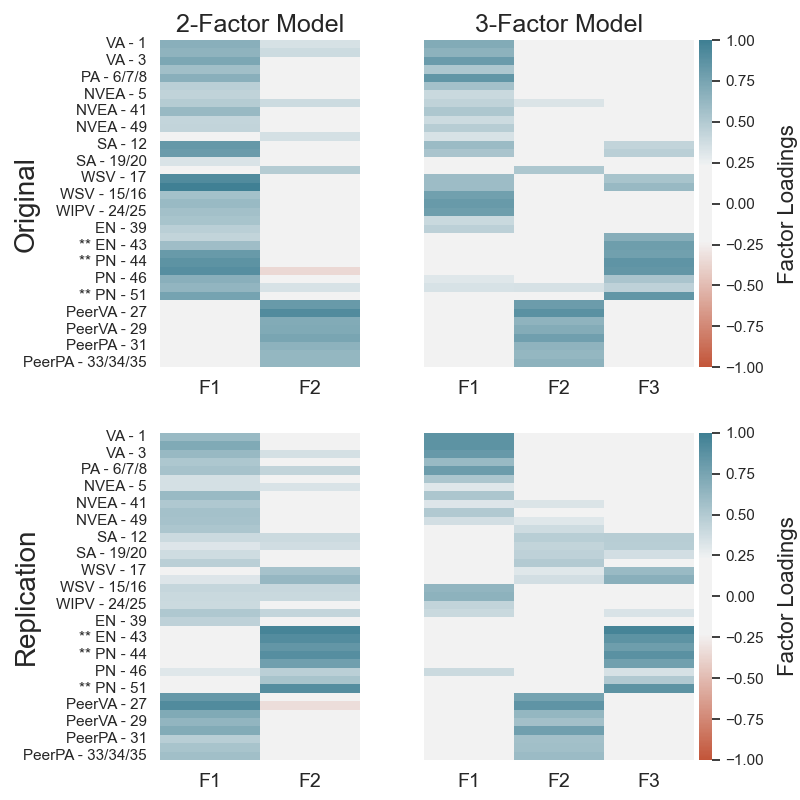
\includegraphics[width=1\textwidth,center]{figures/fig04.png}
    \caption{\normalfont Standardized factor loadings for the 2- and 3-factor solutions produced by the cf-quartimax rotation for original sample (top row) and replication sample (bottom row). \break \small Notes: VA = verbal abuse; PA = physical abuse; NVEA = nonverbal emotional abuse; SA = sexual abuse; EN = emotional neglect; PN = physical neglect; WSV = witnessing sibling violence; WIPV = witnessing inter-parental violence; PeerVA = peer verbal abuse; PeerPA = peer physical abuse. Only factor loadings $\geq$ 0.30 are shown. ** Reverse-scored items.}
    \label{fig:efa_cf}
\end{figure}

The 3-factor solution for each sample were similar. EFA produced a primary maladaptive parenting factor with secondary peer victimization and reverse-scoring factors. (Interestingly, items concerning sexual abuse loaded more strongly on the peer victimization scale in the replication sample, raising some questions about the replicability of the factor structures.) To conclude, the structure of both the 2- and 3-factor exploratory factor models resembled the bifactor S-1 model with two specific factors (model 4), providing further support for that model of the factor structure of the MACE. 

\section{Discussion}

The MACE is a promising measure of childhood maltreatment \citep{georgieva2022systematic}. Despite its increasing popularity, there has been little investigation into the MACE's structural validity \citep{saini2019systematic} leaving unanswered questions about its factor structure and the validity of its total/subscale scores. Here we investigated the factor structure of the MACE, using both confirmatory and exploratory item response modeling, in two independent samples. Bifactor modeling revealed a dominant general maltreatment factor, characterized by uniformly strong loadings across items, and much weaker specific factors. The general factor explained approximately 70\% of the reliable variance in the response data across samples. Moreover, the general factor loadings from the bifactor models largely resembled the corresponding loadings from a unidimensonal model. Together, these results support the conclusion that the MACE is essentially unidimensional. 

We also calculated reliability indices for the MACE total and subscale scores. We found that the MACE total score has excellent reliability and is a valid measure of overall maltreatment. In contrast, we found that virtually no MACE subscale scores were reliable measures of particular types of maltreatment. For all but one of the 10 MACE subscales, the majority of reliable variance in scores was attributable to the general factor. The same was true of deprivation subscale scores, which were also contaminated by a reverse-scoring methods factor. In short, our results further validate the use of the MACE total score, but caution against the use of MACE subscale scores. Indeed, MACE subscale scores seldom reflected their intended construct but instead reflected general maltreatment.

Of the four confirmatory factor models we tested, the most parsimonious and best- fitting was a bifactor S-1 model with a prominent general maltreatment factor and two specific factors measuring peer victimization and reverse-scoring. This model of the MACE factor structure was additionally supported by the exploratory factor analyses, which produced a qualitatively similar partitioning of the items. Thus, it appears the MACE is essentially unidimensional with secondary factors affecting a small subset of items. Interestingly, we found the peer victimization subscale scores to be reliable; a majority of their variance was attributable to the peer victimization factor even after controlling for general maltreatment. It may therefore be appropriate to produce a peer victimization subscale score from the MACE, but additional research is needed to validate this measure.

Our results are consistent with a number of previous studies investigating the factor structure of other childhood maltreatment questionnaires. For example, bifactor models of the Childhood Trauma Questionnaire have also revealed a dominant general maltreatment factor and weaker specific factors \citep{spinhoven2014childhood, stagaki2022mediating}. Similar results were found in recent applications of a bifactor model to the International Child Abuse Screening Tool \citep{meinck2021factor} and the Adverse Childhood Experience questionnaire \citep{dobson2021latent}. Together, these and our current results underscore a challenge in investigating the consequences of childhood maltreatment. When maltreatment experiences tend to co-occur, it is difficult to measure the effects of a particular type of adversity unique from overall maltreatment.  
 
Our results are also worth considering alongside previous studies that used MACE subscale scores to investigate the link between particular types of childhood maltreatment and assorted psychobiological outcomes. For example, researchers have looked at the relationship between MACE subscale scores and risk of depression \citep{gerke2018childhood}, dissociative symptoms, \citep{schalinski2015type}, and cortisol concentration \citep{schalinski2019early}. Still others have used threat and deprivation subscale scores from the MACE to study their associations with cognitive functioning \citep{schalinski2018defining} and hippocampal volume \citep{teicher2018differential}. Our results are clear that these scores chiefly reflect general maltreatment and not particular types of adversity, which presents a challenge for interpreting the conclusions of those studies. It is worth noting that some of these studies attempted to control for general maltreatment by entering all of the MACE subscale scores simultaneously into sophisticated multivariate analyses (e.g. random forest regression). This approach is unsatisfactory for two reasons. First, random forest models can produce spurious results when dealing with collinear predictors \citep{gregorutti2017correlation}. Second, even if one were to properly control for general maltreatment, our results indicate that the remaining reliable variance in most subscale scores is so low as to cast doubt about the utility of these inferences.

The current study revealed other features of the MACE worth highlighting. For example, we identified several sources of DIF in the MACE. We found that across samples women experienced more sexual abuse whereas men experienced more physical abuse by peers. These findings are in line with previous research \citep{radford2013prevalence}. We also identified a number of items with DIF by sample. The cause for this is unclear and may reflect differences in sample population (greater Boston area vs. US \& Canada), study location (in clinic vs. online), recruitment years (early 2010s vs. early 2020s), inclusion criteria (healthy \& unmedicated vs. none), and/or exclusion criteria (none vs. attention checks). The causes and impact of violations of measurement invariance on the MACE require further study. 

We also identified a reverse-scoring methods factor in the MACE. In our view, the most plausible explanation is that, under the \cite{teicher2015maltreatment} scoring procedure, affirmative responses on the regular and reverse-scored items on the MACE represent very different endorsements. For a regular item on the MACE, an endorsement indicates that a person experienced an adverse event during one year of childhood at least. In contrast, an endorsement on a reverse-scored item indicates that a person experienced experienced the absence of a positive event for all 18 years of childhood. Alternative causes of the reverse-scoring factor such as participant confusion, acquiescence, or carelessness \citep{weijters2013reversed} are also possible. Additional research is needed to see if alternative scoring procedures eliminates this factor. 

The current study is not without limitations. The most apparent limitation is that we only studied the dichotomous response data, but not the chronology data that is also collected as part of the MACE. Though we found that the factor structure of the endorsement responses is essentially unidimensional, this may belie more complex patterns present in the maltreatment chronology data. Indeed, longitudinal models of adverse events across childhood --- perhaps using dynamic factor analysis \citep{zhang2007bayesian} --- might be more sensitive to patterns of maltreatment covariation that are lost when collapsing the data into a dichotomous indicator of none vs. any maltreatment. Another possibility is to jointly model the MACE endorsement and chronology data using a multidimensional hurdle model \citep{magnus2021symptom}, which measures both a person's susceptibility to maltreatment (number of maltreatment experiences) and severity of maltreatment (duration of maltreatment experiences). Further research is needed to develop maltreatment scores that integrate the MACE endorsement and chronology data. 

A second limitation is our sample demographics. Though the replication sample increased the overall diversity of our sample with respect to gender and age, other types of diversity are notably lacking. Our combined sample was neither racially nor ethnically diverse. This is important as previous studies have identified DIF for childhood adversity questionnaires by race \citep{rodriguez2019identification}, which raises the question whether similar issues would be found for the MACE in more diverse samples. Moreover, we are not currently able to explain why we found DIF in multiple items by sample membership in the current study. Additional research is needed to study the functioning of the MACE in more diverse samples in order to validate its use in different populations. 

To conclude, the results of the current study show the factor structure of the MACE is essentially unidimensional. Bifactor models revealed that, despite the presence of smaller secondary factors, the majority of reliable variance in the MACE endorsement responses are attributable to a general maltreatment factor. Accordingly, we found that the MACE total score is a reliable and valid of overall maltreatment. In contrast, we found that MACE subscale scores are not reliable measures of particular types of childhood maltreatment; instead they mainly reflect general maltreatment. Moving forward, childhood maltreatment researchers using the MACE (or any other scale) should ensure that any subscale scores used as part of their analyses are reliable, lest they risk drawing spurious inferences. 

\bibliography{main}

\pagebreak
\section{Supplementary materials}

\setcounter{figure}{0}
\setcounter{table}{0}
\renewcommand{\thetable}{S\arabic{table}}
\renewcommand{\thefigure}{S\arabic{figure}}

\subsection*{Additional self-report measures}

In addition to the MACE, participants in both samples completed a number of additional self-report measures. Participants in the original sample completed multiple measures concerning psychiatric symptoms; these have already been reported \citepSM{teicher2015maltreatment}. The participants in the replication sample completed three additional self-report measures all assessing negative symptoms and motivation for rewards. Specifically, participants completed the Motivation and Pleasure scale \citepSM{llerena2013motivation}, the Self-evaluation of Negative Symptoms scale \citepSM{dollfus2016self}, and the revised Behavioral Inhibition / Behavioral Activation scale \citepSM{pagliaccio2016revising}.

Following best practices for online research \citepSM{zorowitz2021inattentive}, several attention checks were embedded in the secondary self-report measures filled out by the replication sample. Specifically, we used infrequency items which are questions for which all  or virtually all attentive participants should provide the same response. Specifically, we used the following questions:

\begin{enumerate}
    \item I'm able to blink my eyes without difficulty. (all endorse)
    \item I was motivated to write Mumfred Mumford's biography. (none endorse)
    \item I worry about the 2001 Cricket World Cup. (none endorse)
    \item Please select "Yes" and then select age "17". (instructed item)
\end{enumerate}

\noindent Prior to conducting the study, the infrequency items were piloted on an independent sample of participants to ensure that they elicited one dominant response. Participants were excluded from analysis if they responded incorrectly to one or more of these items.

%One might question whether it is appropriate to model childhood maltreatment data using common factor models (e.g. bifactor models). The core assumption of these models is that the direction of causality is from the factor to the indicators. That is, variation in item responses are caused by (or reflect) variation in a shared factor. This is in contrast to composite variable models where the direction of causality is reversed; there the indicators cause (or form) the latent variable. Common factor and composite variable models are differentiable in two important ways \citep{bollen1991conventional, bollen2011three}. First, covariation among indicators is expected under a common factor model due to the influence of a shared common factor; conversely, covariation among indicators is not required (though may still occur) under a composite variable model. Second, indicators under the common factor model, but not the composite variable model, are expected to share causal antecedents because they reflect a common source. Multiple authors have argued that adverse childhood experiences should (often) be treated as formative, not reflective \citep{netland2001assessment, layne2010unpacking}. Indeed it is the occurrence of abuse and neglect that defines childhood maltreatment, not the other way around. Moreover, theoretical models of the consequences of childhood maltreatment neither require that adverse experiences covary nor assume they share causal antecedents. 

%For the purposes of explaining patterns of responding on the MACE, we think we are justified in using a common factor model. The vast majority of items on the MACE measure maltreatment by parents or other adults in the home. Thus, the homogeneity of these indicators makes it plausible that they reflect a common source (e.g. parental maltreatment, household dysfunction), as does their pattern of covariation as evidenced by strong loadings onto a common factor. Moreover, there is theoretical support for a model in which a common source like parental maltreatment, itself caused by a diversity of parent level (e.g. emotional lability, impulse control, history of childhood abuse) and child-parent level factors, resulting in a multiple of forms of maltreatment \citep{belsky1993etiology}. This is empirically supported insofar that multiple forms of maltreatment share overlapping risk factors \citep{stith2009risk, mulder2018risk, assink2019risk}. Furthermore, the MACE is a retrospective self-report measure. Prospective and retrospective measures do not have perfect agreement \citep{patten2015retrospective, reuben2016lest}, and thus must reflect other factors related to the participants including individual differences in current state, memory, appraisal, personality, and biases in discloure \citep{susser2012still, reuben2016lest, colman2016consistency}. 

%This in turn raises another question: whether it is reasonable for indicators of parental maltreatment and peer victimization on the MACE to share a common factor. At first blush, one might reasonably assume that the causes of the former would be independent of the causes of the latter. However, there is ample evidence that children who have been maltreated are at greater risk for subsequent peer victimization \citep{bolger2001developmental, benedini2016cycle}. The reasons for this association are manifold. For example, maltreatment may influence a child's sociocognitive development (e.g. attachment style, emotion regulation) in ways that may predispose them to peer victimization \citep{goemans2021child, McCrory2022-cj}. Parental neglect, or the absence of adult supervision, is also a risk factor for peer victimization \citep{lereya2013parenting}, potentially by increasing the likelihood of children participating in higher risk social situations where victimization may take place. Insofar that parental maltreatment is an indirect cause of peer victimization (mediated by a number of complex psychosocial pathways), then we believe we are justified specifying indicators of peer victimization to load in part onto the common factor. This is also highlights the need for future study of the peer victimization factor on the MACE, to better understand how it is related to and distinct from childhood maltreatment by parents and what its downstream consequences are. 

\pagebreak
\subsection*{Supplementary tables \& figures}

\begin{longtable}{P{0.02\linewidth}p{0.7\linewidth}|P{0.05\linewidth}P{0.05\linewidth}P{0.05\linewidth}}
\centering
\# & Item & \multicolumn{3}{c}{Tetrachoric Corr.} \\
\toprule
6 & {\small Intentionally pushed, grabbed, shoved, slapped, pinched, punched or kicked you.} & - & & \\
7 & {\small Hit you so hard that it left marks for more than a few minutes.} & 0.778 & - &  \\
8 & {\small Hit you so hard, or intentionally harmed you in some way, that you received or should have received medical attention.} & 0.702 & 0.758 & - \\
\midrule
9& {\small Spanked you on your buttocks, arms or legs.} & - & \\
10	& {\small Spanked you on your bare (unclothed) buttocks.} & 0.862 & - & \\
11 & {\small Spanked you with an object such as a strap, belt, brush, paddle, rod, etc.} & 0.816 & 0.519 & - \\
\midrule
13 & {\small Touched or fondled your body in a sexual way.} & - \\
14 & {\small Had you touch their body in a sexual way.} & 0.954 & - \\
\midrule
15 & {\small Hit your sibling (stepsibling) so hard that it left marks for more than a few minutes.} &  \\
16 & {\small Hit your sibling (stepsibling) so hard, or intentionally harmed him or her in some way, that he/she received or should have received medical attention.} & 0.966 & - \\
\midrule
19 & {\small Had you touch their body in a sexual way.} & - \\
20 & {\small Actually had sexual intercourse (oral, anal or vaginal) with you.} & 0.909 & - \\
\midrule
21 & {\small Saw adults living in the household push, grab, slap or throw something at your mother (stepmother, grandmother).} & - \\
22 & {\small Saw adults living in the household hit your mother, stepmother, or grandmother so hard that it left marks for more than a few minutes.} & 0.920 & -  \\
23 & {\small Saw adults living in the household hit your mother, stepmother, or grandmother so hard, or intentionally harm her in some way, that she received or should have received medical attention.} & 0.808 & 0.934 & - \\
\midrule
24 & {\small Saw adults living in the household push, grab, slap or throw something at your father (stepfather, grandfather).} &  \\
25 & {\small Saw adults living in the household hit your father, stepfather, or grandfather so hard that it left marks for more than a few minutes.} & 0.900 & -\\
\midrule
33 & {\small Peers intentionally pushed, grabbed, shoved, slapped, pinched, punched, or kicked you.} & - \\
34 & {\small Peers hit you so hard that it left marks for more than a few minutes.} & 0.829 & - \\
35 & {\small Peers hit you so hard, or intentionally harmed you in some way, that you received or should have received medical attention.} & 0.723 & 0.907 & - \\
\midrule
36 & {\small Peers forced you to engage in sexual activity against your will.} &  - & \\
37 & {\small Peers forced you to do things sexually that you did not want to do.} & 0.975 & - \\
\bottomrule
\caption{\normalfont The 12 item pairs and triplets in the MACE characterized by response dependence. The tetrachoric correlation (averaged over samples) for each pair of items in a set is presented in tandem with the item wording.}
\label{tab:dependence}
\end{longtable}

\begin{table}[H]
    \centering
    \begin{tabular}{llccccc}
    \toprule
    Sample      & Model    & $\chi^2$ ($df$) & RMSEA & CFI & TLI & SRMR \\
    \midrule
    Original    & 2-factor & 1876 (664) & 0.049 & 0.962 & 0.957 & 0.122 \\
                & 3-factor & 1237 (627) & 0.036 & 0.981 & 0.977 & 0.105 \\
    \midrule
    Replication & 2-factor & 1737 (664) & 0.052 & 0.961 & 0.957 & 0.108 \\
                & 3-factor & 1227 (627) & 0.040 & 0.978 & 0.974 & 0.097 \\
    \bottomrule
    \end{tabular}
    \caption{\normalfont Fit statistics for the exploratory factor models by sample. Notes: RMSEA = root mean square error of approximation; CFI = comparative fit index; TLI = Tucker-Lewis index; SRMR = standardized root mean square residual.}
    \label{tab:efa_diagnostics}
\end{table}

\begin{figure}[H]
    \centering
    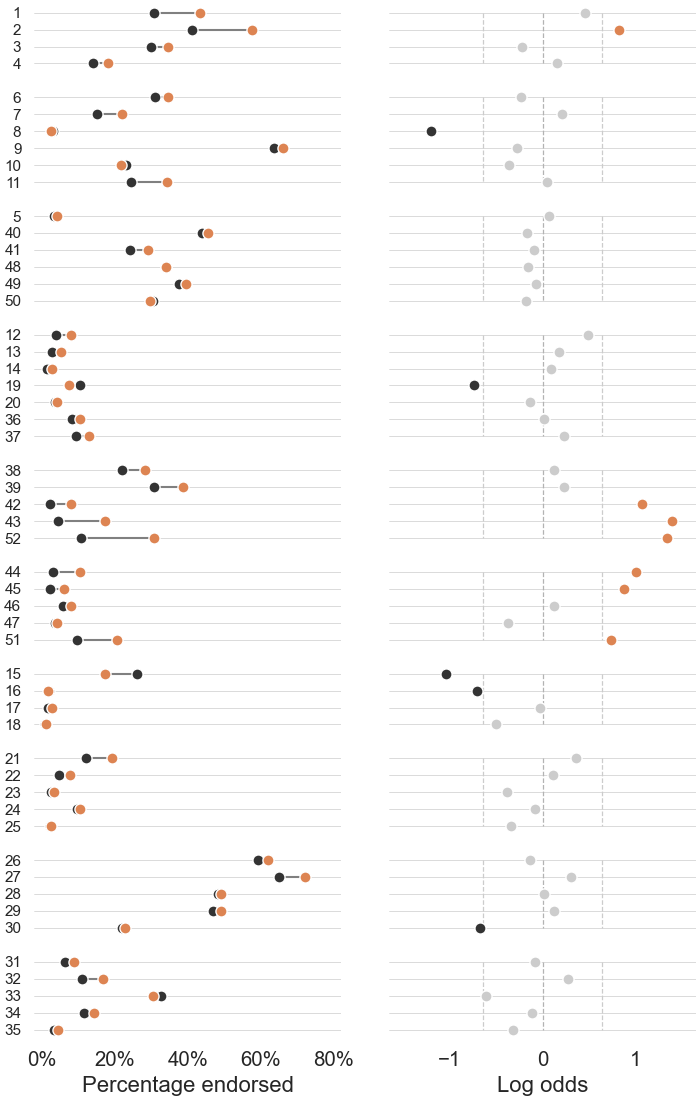
\includegraphics[width=0.82\textwidth,center]{figures/figS01.png}
    \caption{\normalfont \begin{spacing}{1.25} Differential item functioning by sample. (A) Proportions of participants endorsing having experienced a maltreatment event by study sample. (B) The log odds that the proportion of endorsements are larger in one or the other sample. Dotted lines indicate the threshold for large DIF recommended by \cite{hidalgo2014binary}. ** Reverse-scored items. \end{spacing}}
    \label{fig:dif_study}
\end{figure}

\begin{figure}[H]
    \centering
    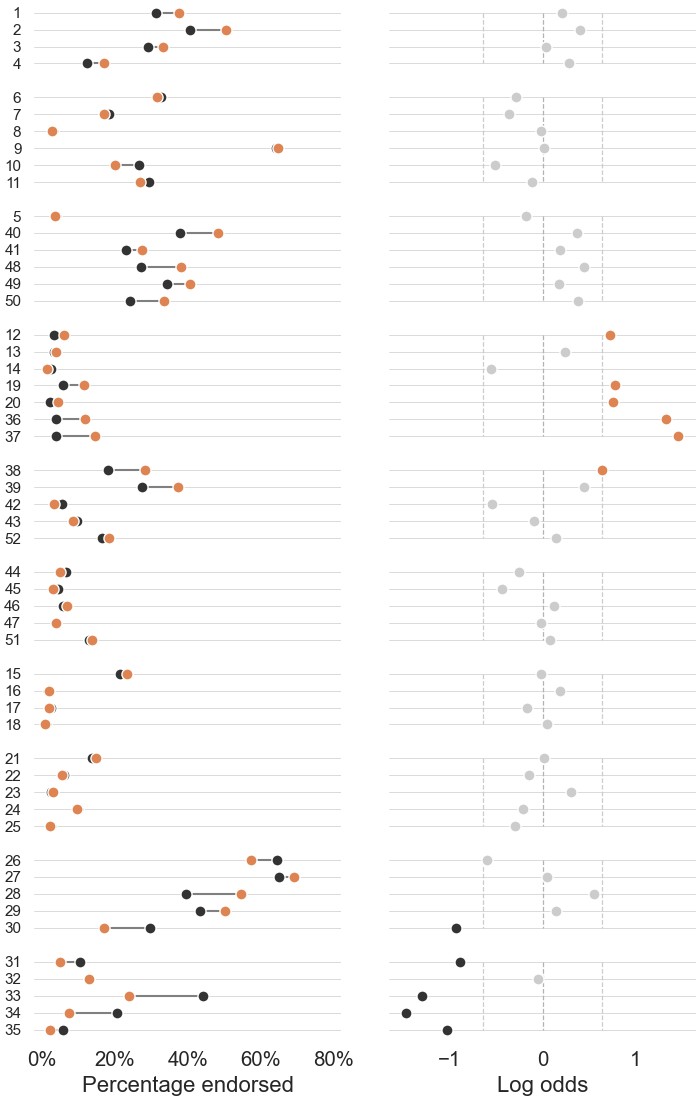
\includegraphics[width=0.82\textwidth,center]{figures/figS02.png}
    \caption{\normalfont \begin{spacing}{1.25} Differential item functioning by gender. (A) Proportions of participants endorsing having experienced a maltreatment event by study gender. (B) The log odds that the proportion of endorsements are larger in one or the other gender. Dotted lines indicate the threshold for large DIF recommended by \cite{hidalgo2014binary}. ** Reverse-scored items. \end{spacing}}
    \label{fig:dif_gender}
\end{figure}

\begin{figure}[H]
    \centering
    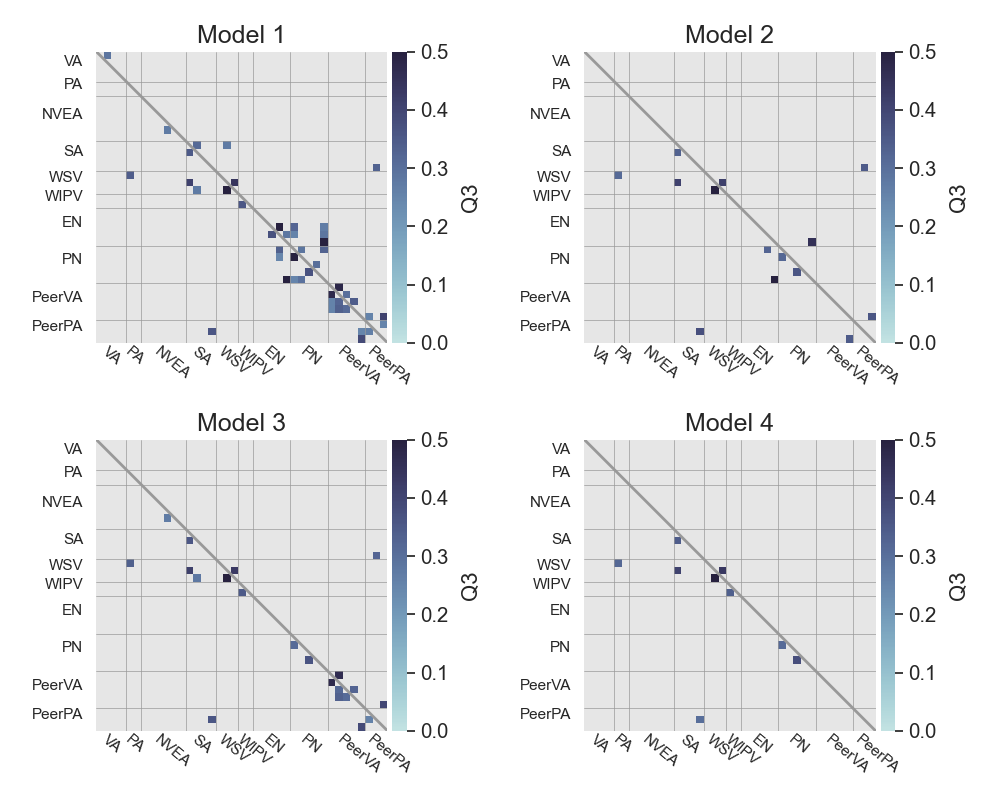
\includegraphics[width=1.05\textwidth,center]{figures/figS03.png}
    \caption{\normalfont Yen's $Q_3$ values for item pairs exceeding the 99\% percentile critical value for each confirmatory item response model. Cells beneath the gray diagonal line correspond to the original sample, whereas cells above the line correspond to the replication sample. Notes: VA = verbal abuse; PA = physical abuse; NVEA = nonverbal emotional abuse; SA = sexual abuse; EN = emotional neglect; PN = physical neglect; WSV = witnessing sibling violence; WIPV = witnessing inter-parental violence; PeerVA = peer verbal abuse; PeerPA = peer physical abuse.}
    \label{fig:local_dependence}
\end{figure}

\begin{figure}[H]
    \centering
    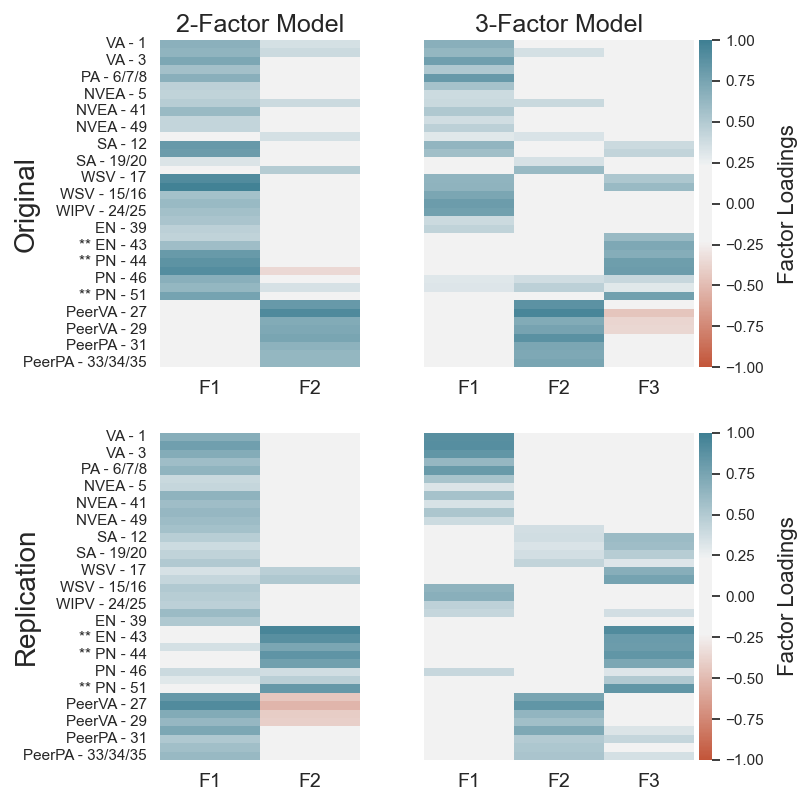
\includegraphics[width=1\textwidth,center]{figures/figS04.png}
    \caption{\normalfont Standardized factor loadings for the 2- and 3-factor solutions produced by the geomin rotation for original sample (top row) and replication sample (bottom row). Notes: VA = verbal abuse; PA = physical abuse; NVEA = nonverbal emotional abuse; SA = sexual abuse; EN = emotional neglect; PN = physical neglect; WSV = witnessing sibling violence; WIPV = witnessing inter-parental violence; PeerVA = peer verbal abuse; PeerPA = peer physical abuse. Only factor loadings $\geq$ 0.30 are shown. ** Reverse-scored items.}
    \label{fig:efa_geomin}
\end{figure}

\bibliographystyleSM{apalike}
\bibliographySM{main}

\end{document}
